\section{Experimental Evaluation}

To evaluate the performance of Viscous, we perform several experiments over \texttt{Mininet} network emulation platform. We have used two different network topologies for emulation, as shown in Fig.~\ref{fig:experimentalTopology1} (Topology-1) and Fig.~\ref{fig:experimentalTopology2} (Topology-2). In Topology-1, $H1$ has multiple interfaces, but $H2$ has a single interface; whereas in Topology-2, both $H1$ and $H2$ have multiple interfaces. In these two topologies, $H1$ and $H2$ act as the Viscous server and the Viscous client, respectively, or vice-versa. Rest of the hosts generate background traffic; and we evaluate the performance of Viscous both in the presence as well as in the absence of background traffic.  We compare the performance of Viscous with following protocols;
\begin{enumerate}
	\item[(i)] TCP: We have used TCP Cubic with the optimizations proposed in~\cite{google-long-initcwnd}, where as initial congestion window size of $10$ is used to avoid network underutilization for short-lived flows. 
	\item[(ii)] MPTCP: We have used Linux MPTCP kernel version 0.91 for our implementation.
	\item [(iii)] QUIC: We have compared Viscous with QUIC implementation provided by \texttt{libquic}\footnote{\url{https://github.com/devsisters/libquic} (last accessed: April 25, 2017)}. 
\end{enumerate}

\begin{figure}[!ht]
	\centering
	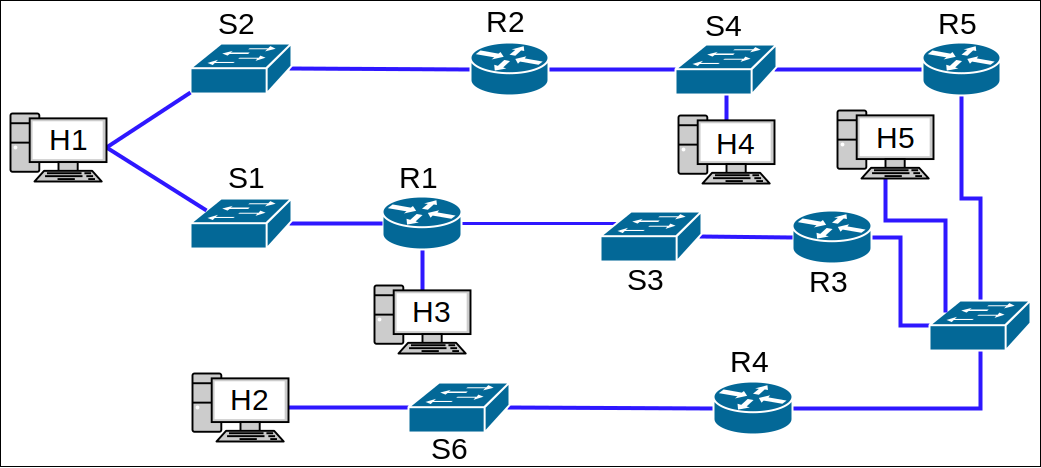
\includegraphics[width=0.7\linewidth]{img/experimentalTopology1}
	\caption{Topology 1: One of the end hosts has a single interface}
	\label{fig:experimentalTopology1}
\end{figure}

\begin{figure}[!ht]
	\centering
	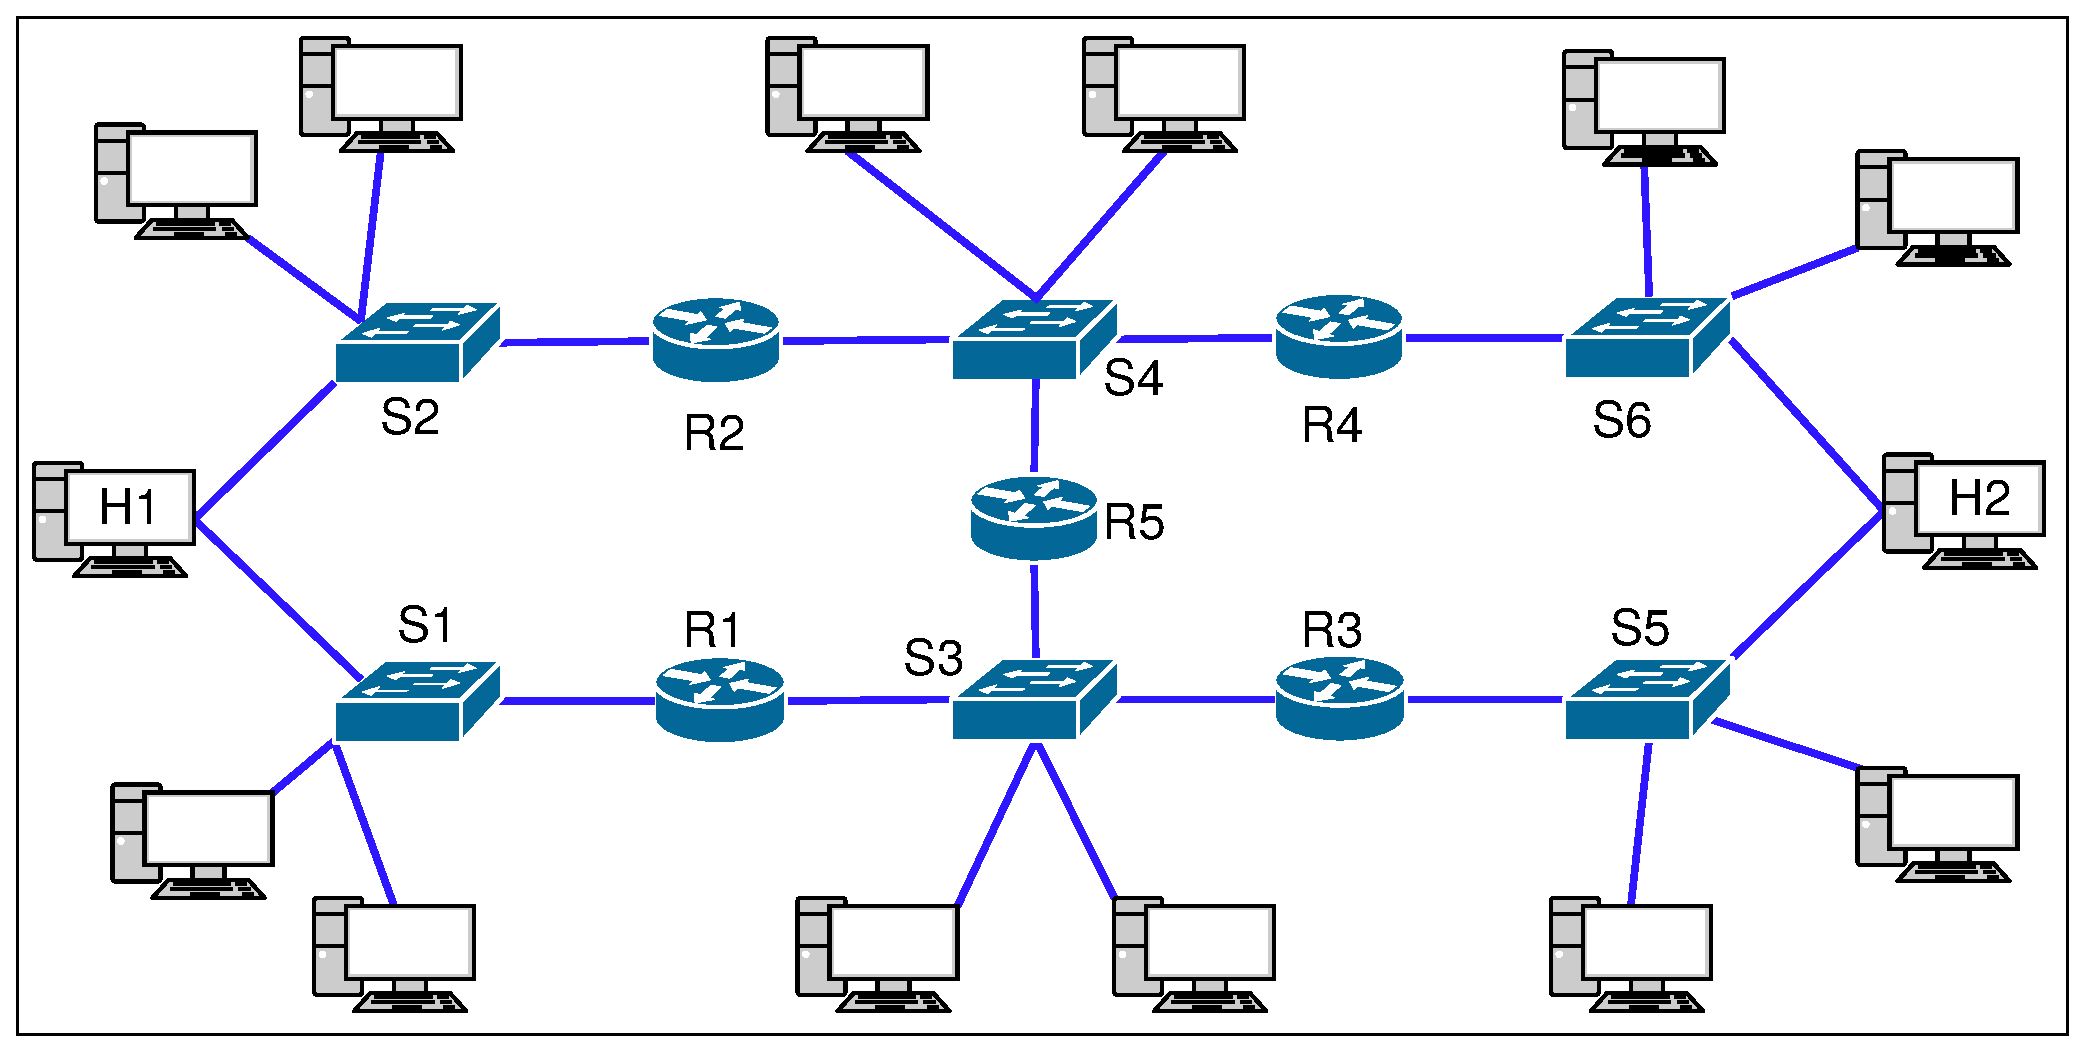
\includegraphics[width=0.7\linewidth]{img/experimentalTopology2}
	\caption{Topology 2: Both the end hosts have two interfaces}
	\label{fig:experimentalTopology2}
\end{figure}



\subsection{Experimental Setup}
The various hardware and operating system level parameters used in our experimental setup are as follows. 
\begin{itemize}
    \item \textbf{System configurations}: We have used Oracle VitualBox to create virtual machines which have been configured with \texttt{Mininet} kernel to support network interface virtualization. The guest machine configuration is as follows -- single core Intel i7-5500U 64bit CPU with clock speed of 2.40 GHz, RAM: 8GB. The host machine configuration is as follows -- Intel Genuin i7-5500U 64bit CPU with clock speed of 2.40GHz, RAM: 8GB with 250GB Solid State Drive.
    \item \textbf{Mininet}: Version 2.2.2 of \texttt{Mininet} kernel have been used to develop our test setup.
    \item \textbf{Kernel}: We have used the Linux kernel version 4.1.38.mptcp, which is patched with the MPTCP implementation.
    \item \textbf{MPTCP}: We have used MultiPath TCP version 0.91 for comparing the performance of Viscous with MPTCP.
    \item \textbf{Operating System}: In our virtual machine configurations for test setup, the guest operating system is Ubuntu 14.04.4 LTS, whereas the host operating system is Ubuntu 16.04.1 LTS. 
\end{itemize}
We setup the link bandwidths for different paths in the topologies as follows. In Topology-1, the two paths from the two interfaces of the host $H1$ up to the common point has a bandwidth of $50$ Mbps, and from the common point to the interface of the host $H2$ has a bandwidth of $100$ Mbps. For Topology-2, all the links have a link bandwidth of $100$ Mbps. 
 
Next we present the results and observations from various test scenarios as performed over the two topologies. 

\subsection{Experiment 1 (Performance over Topology-1 without any Background Traffic)}
\label{sub:experiment1}
In this experiment, we have explored the performance of \acrshort{quic}, \acrshort{tcp}, \acrshort{mptcp} and Viscous for a large numbers of short-lived flows, when there are no background flows. Therefore, the congestion in the network is generated by a single type of flow. This experiment has been performed over Topology-1. In Topology-1, there are two paths between $H1$ and $H2$, however $H2$ has a single interface. Here, we vary the RTT of the two paths from $16$ms to $320$ms, and observe the performance of the four protocols for end-to-end data transport. For every RTT setup, we have sent flows using multiple parallel threads to generate multiple simultaneous flows. For each thread, we have generated $100$ back-to-back flows; and have varied the flow duration based on an exponential distribution with mean flow duration of $25$ seconds. The number of parallel threads those generate the simultaneous flows have been varied from $1$ to $20$.  
%
%Overall delays in each path are varied from 16ms to 320ms. For each delay level, we have sent flows using multiple threads. In each thread, we sent 100 back-to-back short-lived flows. Data sizes for each flow are in exponential distribution \noteam{I forgot the parameters. I will add it later}. We vary the number of threads from 1 to 20. We compared the time required to complete the flows in Fig.~\ref{fig:exp6_time}.

%\begin{figure}[!t]
%	\captionsetup[subfigure]{}
%	\begin{center}
%		\subfloat[\label{fig:exp6_time_16}RTT=16ms]{
%			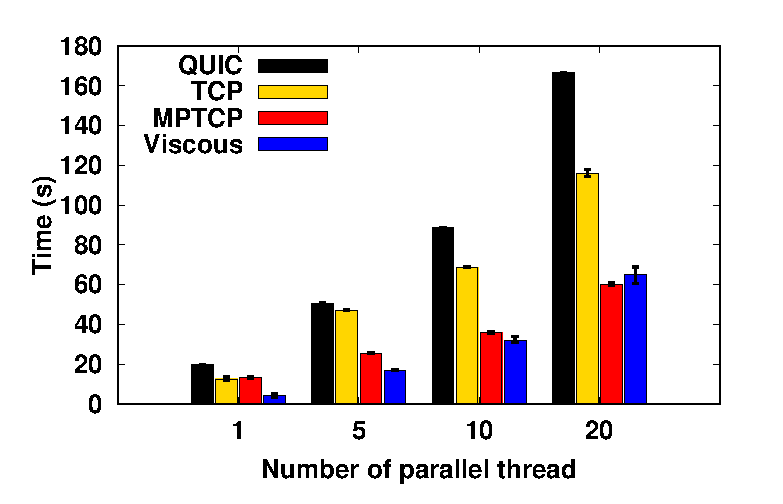
\includegraphics[width=0.24\linewidth]{img/exp6/time_elapsed_1}
%		}
%		\subfloat[\label{fig:exp6_time_80}RTT=80ms]{
%			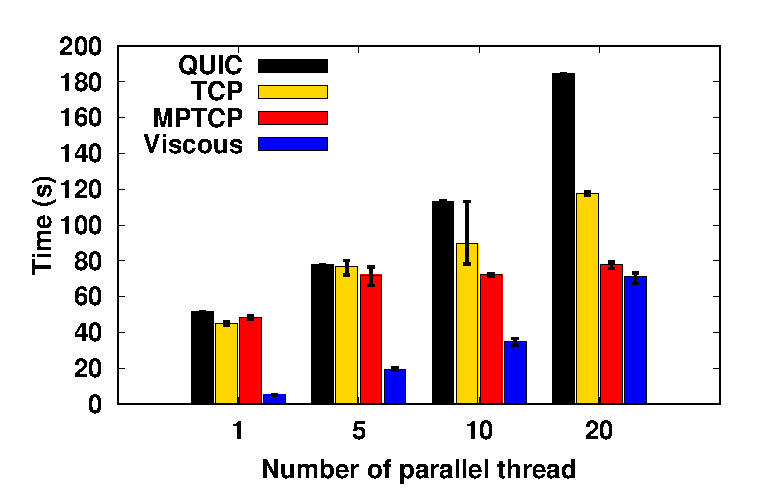
\includegraphics[width=0.24\linewidth]{img/exp6/time_elapsed_5}
%		}
%		\subfloat[\label{fig:exp6_time_160}RTT=160ms]{
%			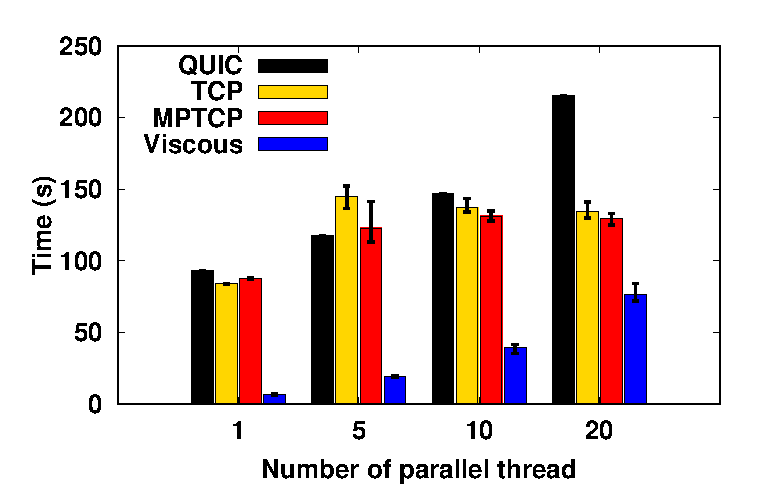
\includegraphics[width=0.24\linewidth]{img/exp6/time_elapsed_10}
%		}
%		\subfloat[\label{fig:exp6_time_320}RTT=320ms]{
%			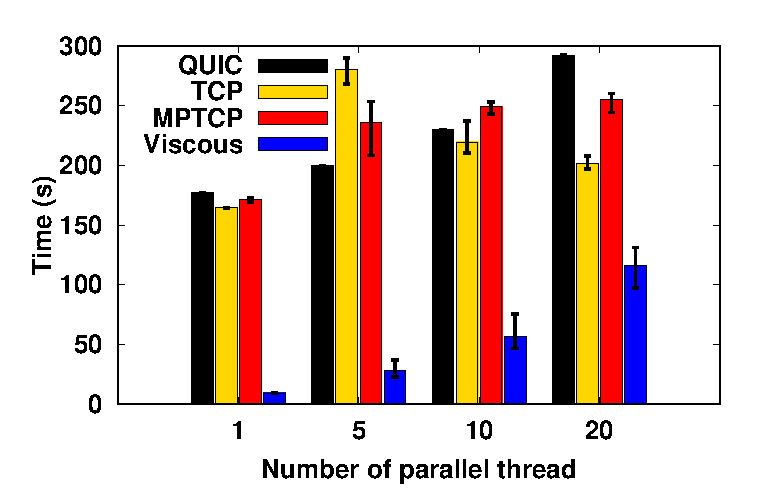
\includegraphics[width=0.24\linewidth]{img/exp6/time_elapsed_20}
%		}
%		\caption{\label{fig:exp6_time} Experiment 1: Flow Completion Time over Topology-1 without Background Flows}
%	\end{center}
%\end{figure}
\begin{figure}[!t]
    \begin{center}
        \begin{minipage}{0.45\linewidth}
            \centering
            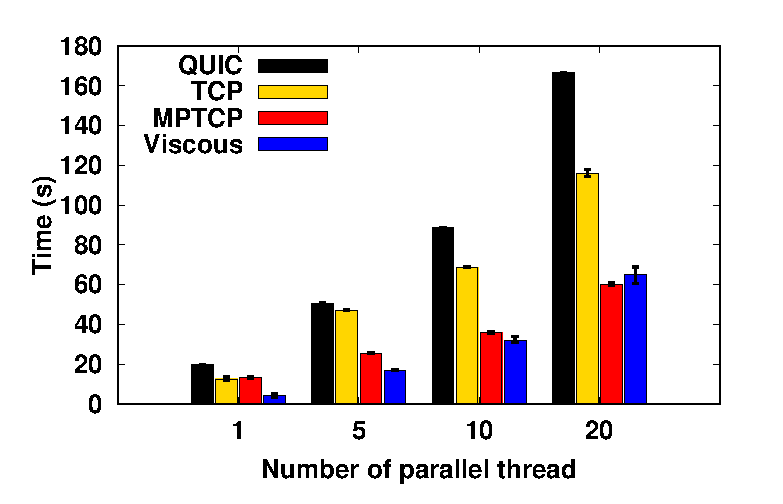
\includegraphics[width=\linewidth]{img/exp6/time_elapsed_1}
            \label{fig:exp6_time_16}
            \subcaption{RTT=16ms}
        \end{minipage}
        \begin{minipage}{0.45\linewidth}
            \centering
            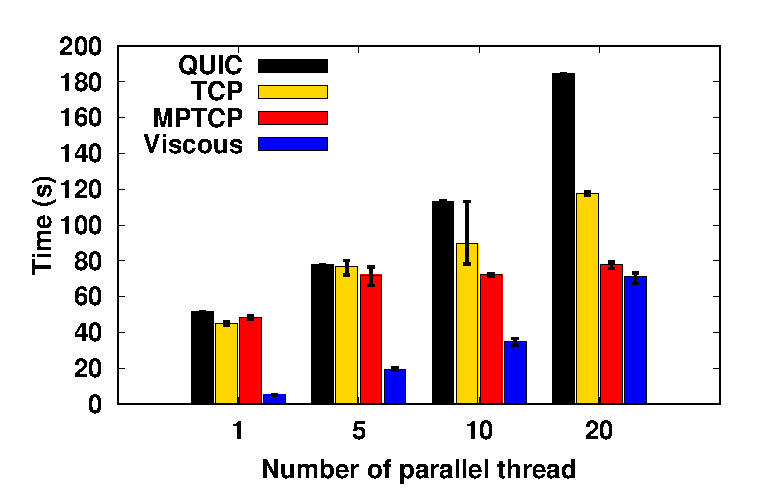
\includegraphics[width=\linewidth]{img/exp6/time_elapsed_5}
            \label{fig:exp6_time_80}
            \subcaption{RTT=80ms}
        \end{minipage}
        \begin{minipage}{0.45\linewidth}
            \centering
            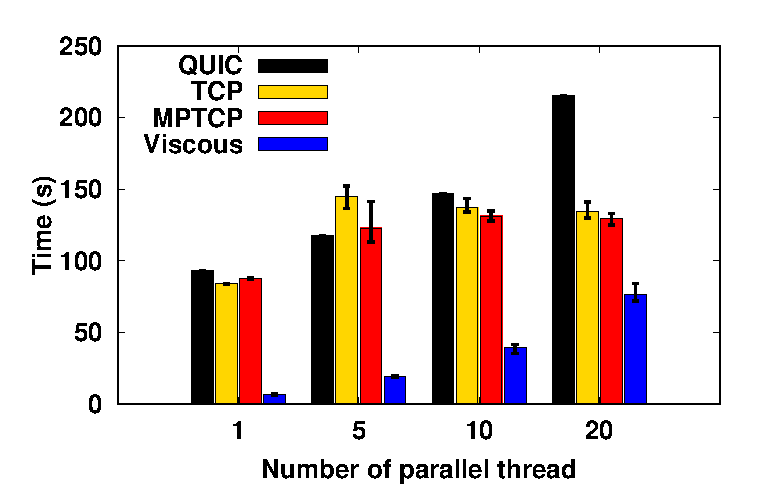
\includegraphics[width=\linewidth]{img/exp6/time_elapsed_10}
            \label{fig:exp6_time_160}
            \subcaption{RTT=160ms}
        \end{minipage}
        \begin{minipage}{0.45\linewidth}
            \centering
            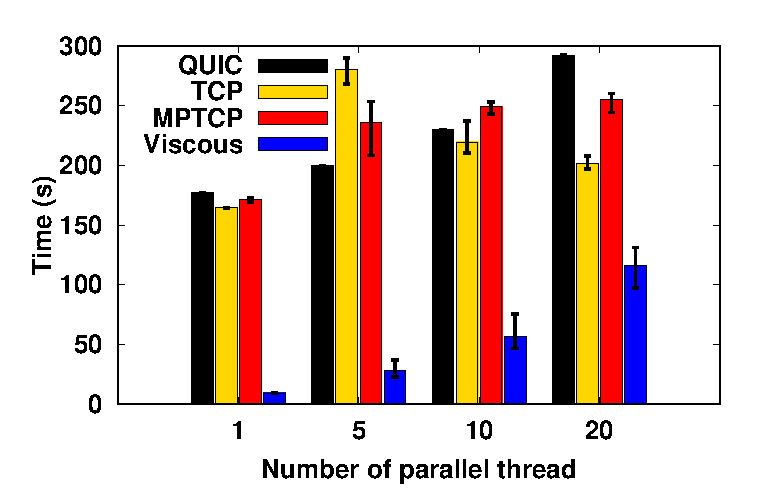
\includegraphics[width=\linewidth]{img/exp6/time_elapsed_20}
            \label{fig:exp6_time_320}
            \subcaption{RTT=320ms}
        \end{minipage}
        \caption{\label{fig:exp6_time}Experiment 1: Flow Completion Time over Topology-1 without Background Flows}
    \end{center}
\end{figure}

\begin{figure}[!t]
	\centering
	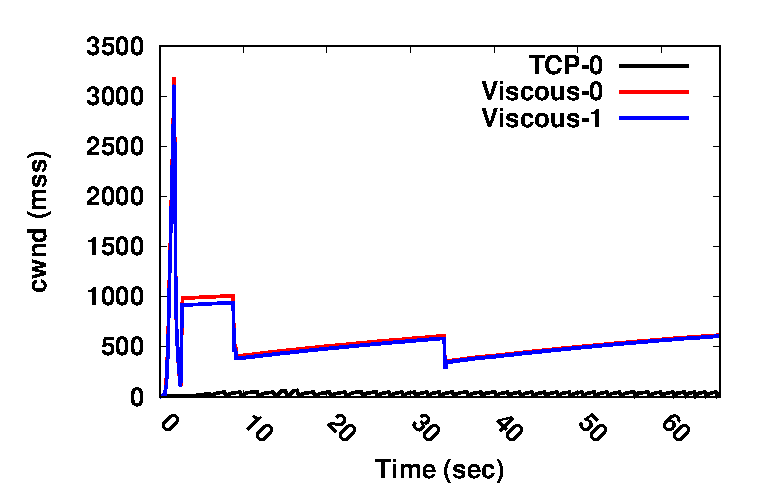
\includegraphics[width=0.5\linewidth]{img/exp6/cwnd_sample1_5_20}
	\caption{Experiment 1: Congestion Window Evolution}
	\label{fig:exp6_cwnd}
\end{figure}

First, we observe the average flow completion time for all the flows over Topology-1 without any background traffic, as shown in Fig.~\ref{fig:exp6_time}. From the figure, we can see that Viscous performs much better when multiple short-lived flows are transferred over the network. QUIC in this scenario does not perform good. Although QUIC can multiplex multiple flows coming from the application layer, it maintains flow specific congestion window, resulting in a slow start problem for the flows. Further, QUIC fails to utilize multiple interfaces available in the network which is one of the main reasons behind its poor performance over the test topology. MPTCP suffers from the path imbalance problem as discussed earlier, and TCP Cubic can not utilize multi-homing capacity for the flows. To analyze the effect of short-lived flows, we compare the congestion window evolution for TCP and Viscous for a specific case, as given in Fig.~\ref{fig:exp6_cwnd}, when RTT=$16$ ms and number of parallel thread = $5$. We observe that the average congestion window for TCP is significantly less. The congestion window evolutions for Viscous along the two paths have been shown (Viscous-0 and Viscous-1), and in both the paths, Viscous can achieve a significant higher values of the congestion window. Consequently, Viscous sub-flows can utilize the available bandwidth at the paths in a significantly better way for multiplexed short-lived flows. 

%
%
%it is clear that Viscous performs much better for multiple short flows. \acrshort{quic} is worse than everyone else. Even normal \acrshort{tcp} connection. We could not be able to collect any other information from \acrshort{quic}. For lower delay and a larger number of threads, \acrshort{mptcp} may have performed slightly better than Viscous (Thread 20 at Fig.~\ref{fig:exp6_time_16}). \acrshort{tcp} and \acrshort{mptcp} is suffering because it needs to setup connection for each flow and starts congestion window ($cwnd$) size from initial congestion window (which is ten mss for this setup). In Fig.~\ref{fig:exp6_cwnd}, we plot $cwnd$ evolution of \acrshort{tcp} and Viscous. Here we can see that for Viscous $cwnd$ grows normally. It crosses the slow-start phase and continues in congestion avoidance phase. However, for \acrshort{tcp} it is hardly visible.

%\begin{figure*}[!t]
%	\captionsetup[subfigure]{}
%	\begin{center}
%		\subfloat[\label{fig:exp6_goodput_16}RTT=16ms]{
%			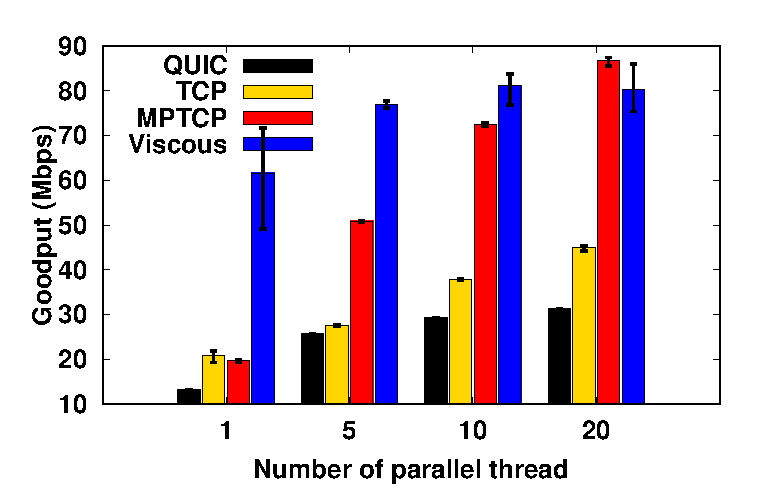
\includegraphics[width=0.24\linewidth]{img/exp6/goodput_1}
%		}
%		\subfloat[\label{fig:exp6_goodput_80}RTT=80ms]{
%			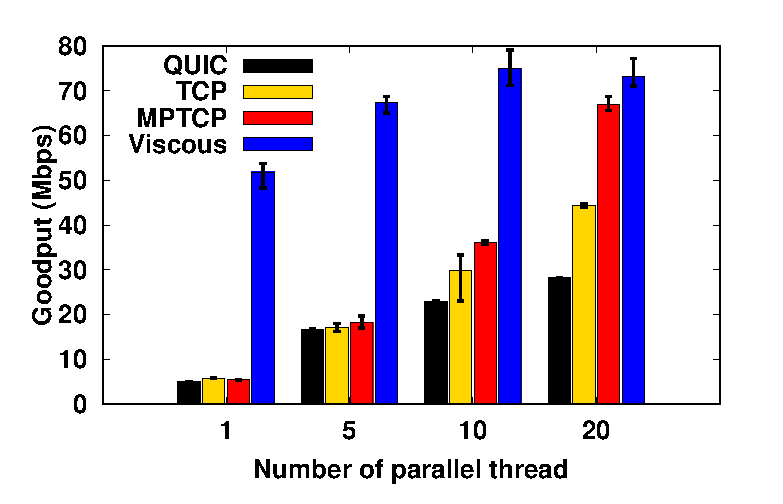
\includegraphics[width=0.24\linewidth]{img/exp6/goodput_5}
%		}
%		\subfloat[\label{fig:exp6_goodput_160}RTT=160ms]{
%			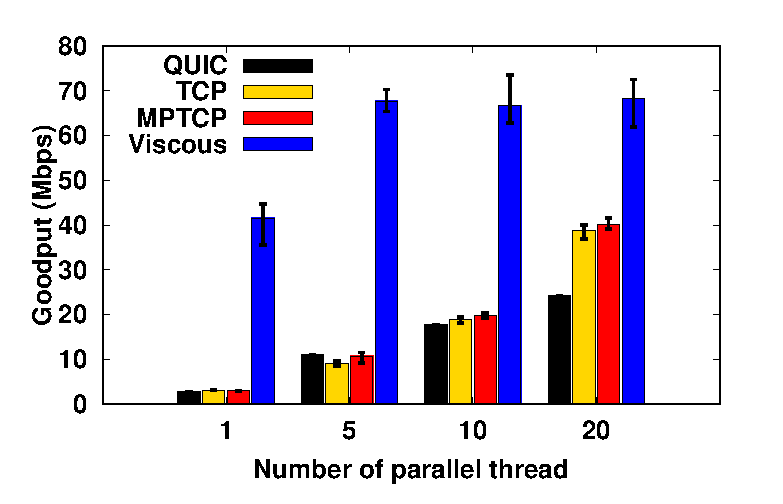
\includegraphics[width=0.24\linewidth]{img/exp6/goodput_10}
%		}
%		\subfloat[\label{fig:exp6_goodput_320}RTT=320ms]{
%			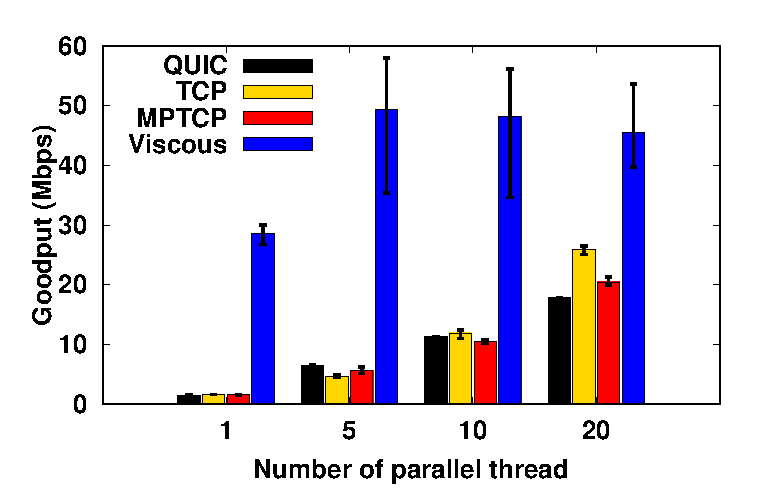
\includegraphics[width=0.24\linewidth]{img/exp6/goodput_20}
%		}
%		\caption{\label{fig:exp6_goodput}Experiment 1: Goodput over Topology-1 without Background Flows}
%	\end{center}
%\end{figure*}

\begin{figure}[!t]
    \begin{center}
        \begin{minipage}{0.45\linewidth}
            \centering
            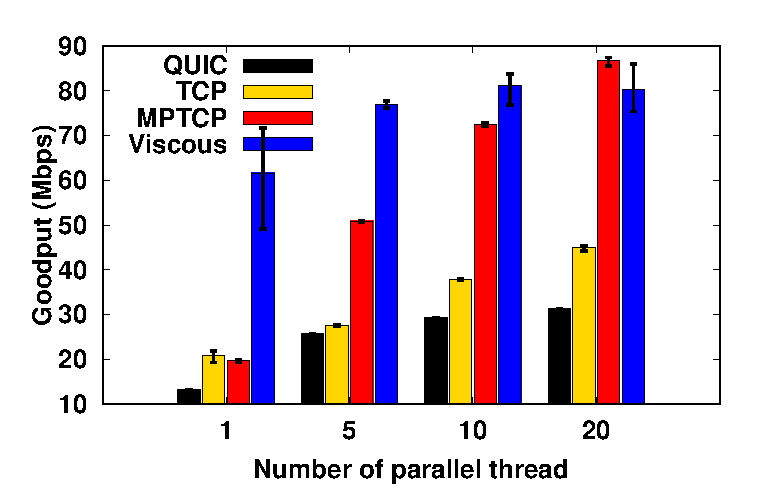
\includegraphics[width=\linewidth]{img/exp6/goodput_1}
            \label{fig:exp6_goodput_16}
            \subcaption{RTT=16ms}
        \end{minipage}
        \begin{minipage}{0.45\linewidth}
            \centering
            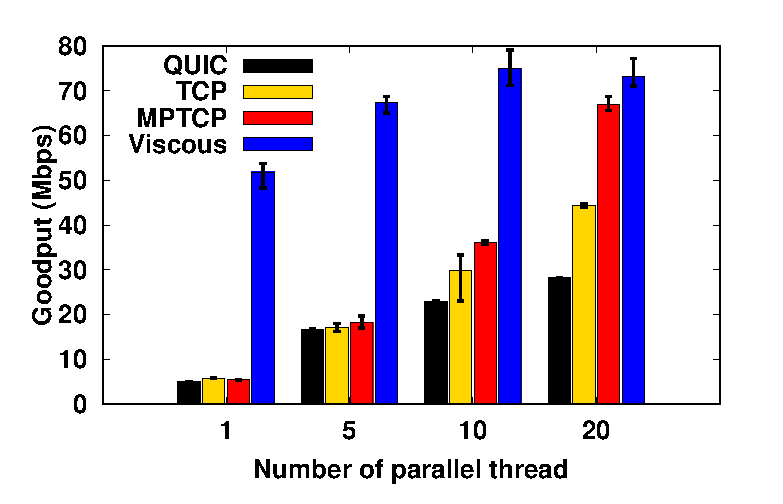
\includegraphics[width=\linewidth]{img/exp6/goodput_5}
            \label{fig:exp6_goodput_80}
            \subcaption{RTT=80ms}
        \end{minipage}
        \begin{minipage}{0.45\linewidth}
            \centering
            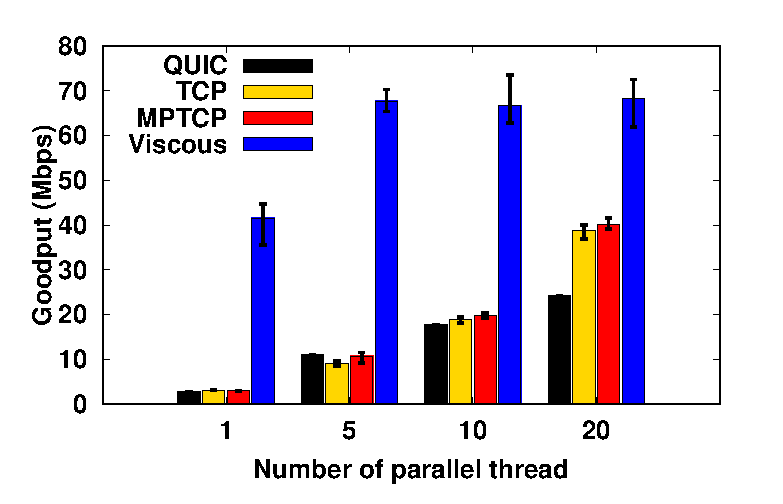
\includegraphics[width=\linewidth]{img/exp6/goodput_10}
            \label{fig:exp6_goodput_160}
            \subcaption{RTT=160ms}
        \end{minipage}
        \begin{minipage}{0.45\linewidth}
            \centering
            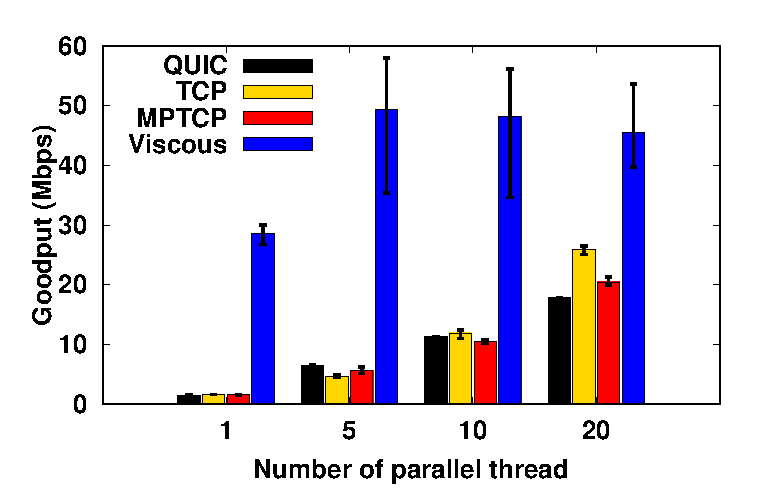
\includegraphics[width=\linewidth]{img/exp6/goodput_20}
            \label{fig:exp6_goodput_320}
            \subcaption{RTT=320ms}
        \end{minipage}
        \caption{\label{fig:exp6_goodput}Experiment 1: Goodput over Topology-1 without Background Flows}
    \end{center}
\end{figure}

Next, we observe the average goodput of the flows for the four different protocols under the same scenario, as shown in Fig.~\ref{fig:exp6_goodput}. Similar to the flow completion time, we observe that the goodput of Viscous is higher than all other protocols. Viscous can utilize the capacity of multiple paths through flow multiplexing and maintaining connection specific congestion window evolution over the time; and therefore it attains higher goodput compared to other competing end-to-end protocols. Further, we observe that the goodput for Viscous is significantly boosted up compared to other protocols, when RTT of the paths is high. This indicates that Viscous overshoots the performance compared to other protocols when network condition is poor. QUIC, TCP and MPTCP can not cope up with the poor network condition, whereas Viscous can effectively utilize the available capacity under all the scenarios. The reason behind this better performance is the Viscous channel scheduler, that uses a self-clocking mechanism to schedule and trigger the transmissions over multiple channels based on the ACK packets. This self-clocking helps in proper utilization of the channels even under poor RTT conditions. 


\subsection{Experiment 2 (Performance over Topology-1 in the Presence of Background Flows)}

\begin{figure}[!t]
	\begin{center}
		\begin{minipage}{0.45\linewidth}
			\centering
			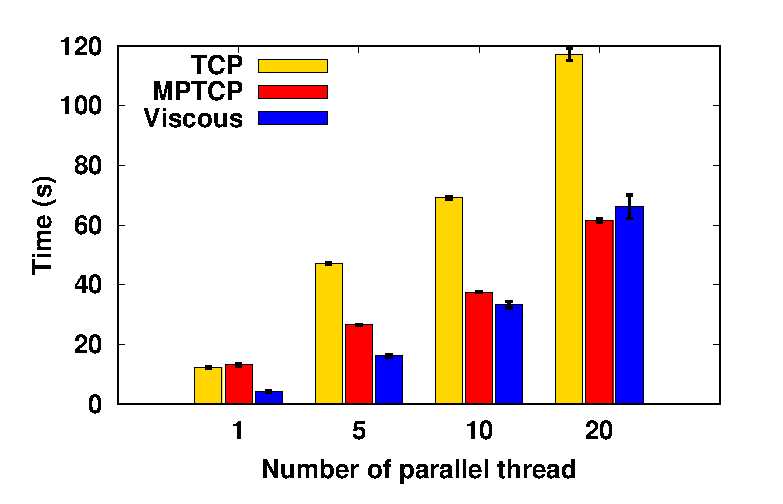
\includegraphics[width=\linewidth]{img/exp7/time_elapsed_1}
			\label{fig:exp7_time_16}
			\subcaption{RTT=16ms}
		\end{minipage}
		\begin{minipage}{0.45\linewidth}
			\centering
			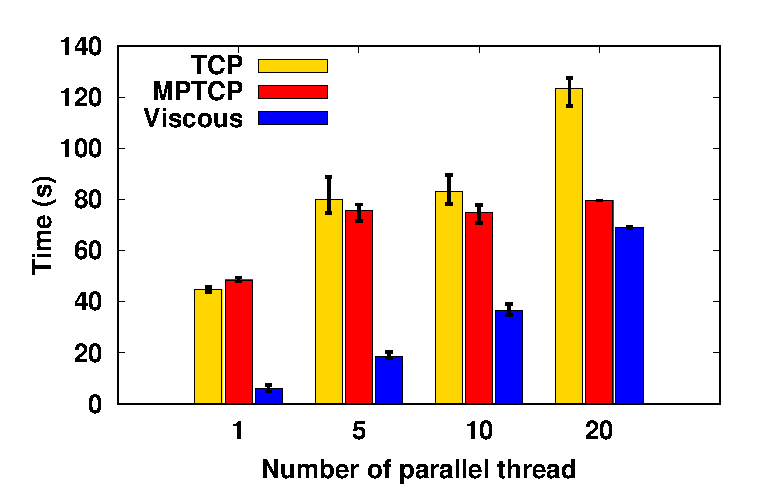
\includegraphics[width=\linewidth]{img/exp7/time_elapsed_5}
			\label{fig:exp7_time_80}
			\subcaption{RTT=80ms}
		\end{minipage}
		\begin{minipage}{0.45\linewidth}
			\centering
			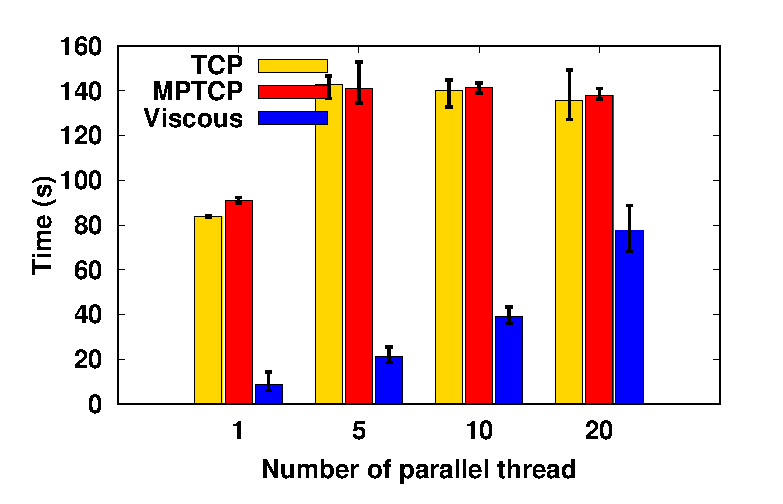
\includegraphics[width=\linewidth]{img/exp7/time_elapsed_10}
			\label{fig:exp7_time_160}
			\subcaption{RTT=160ms}
		\end{minipage}
		\begin{minipage}{0.45\linewidth}
			\centering
			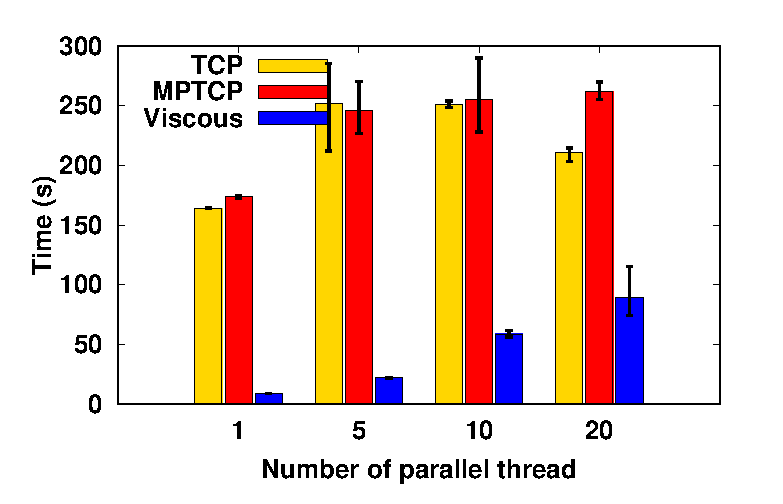
\includegraphics[width=\linewidth]{img/exp7/time_elapsed_20}
			\label{fig:exp7_time_320}
			\subcaption{RTT=320ms}
		\end{minipage}
		\caption{\label{fig:exp7_time}Experiment 2: Flow Completion Time over Topology-1 with Background Traffic}
	\end{center}
\end{figure}

\begin{figure}[!t]
	\centering
	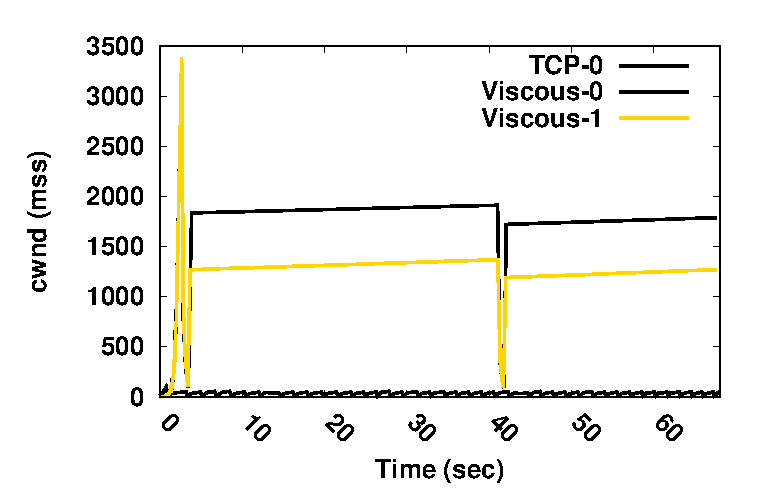
\includegraphics[width=0.5\linewidth]{img/exp7/cwnd_sample2_10_20}
	\caption{Experiment 2: Congestion window evolution}
	\label{fig:exp7_cwnd}
\end{figure}


\begin{figure}[!t]
	\begin{center}
		\begin{minipage}{0.45\linewidth}
			\centering
			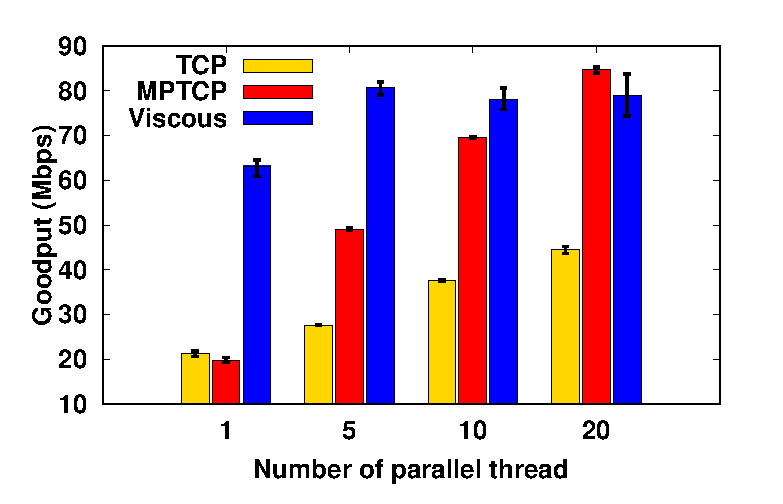
\includegraphics[width=\linewidth]{img/exp7/goodput_1}
			\label{fig:exp7_goodput_16}
			\subcaption{RTT=16ms}
		\end{minipage}
		\begin{minipage}{0.45\linewidth}
			\centering
			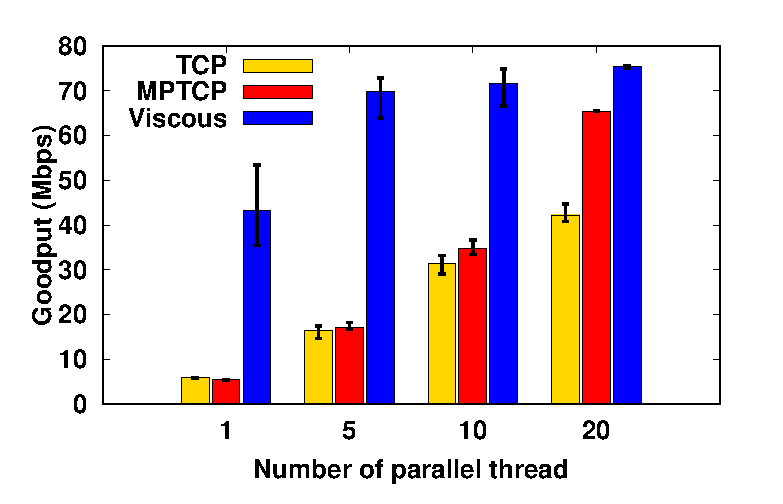
\includegraphics[width=\linewidth]{img/exp7/goodput_5}
			\label{fig:exp7_goodput_80}
			\subcaption{RTT=80ms}
		\end{minipage}
		\begin{minipage}{0.45\linewidth}
			\centering
			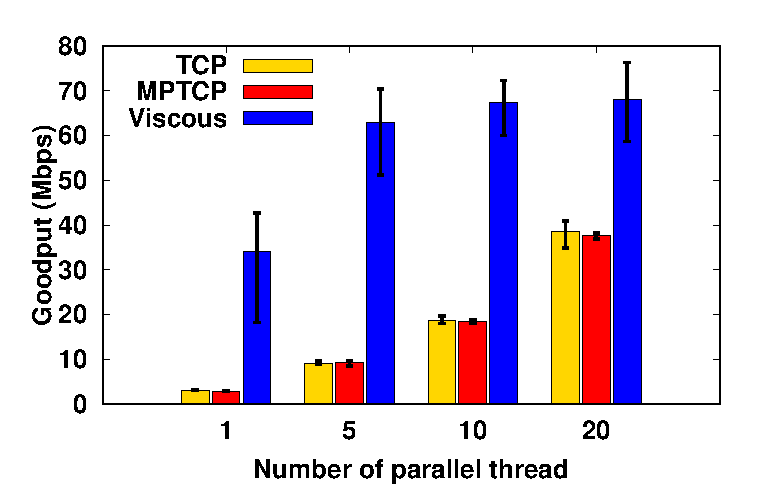
\includegraphics[width=\linewidth]{img/exp7/goodput_10}
			\label{fig:exp7_goodput_160}
			\subcaption{RTT=160ms}
		\end{minipage}
		\begin{minipage}{0.45\linewidth}
			\centering
			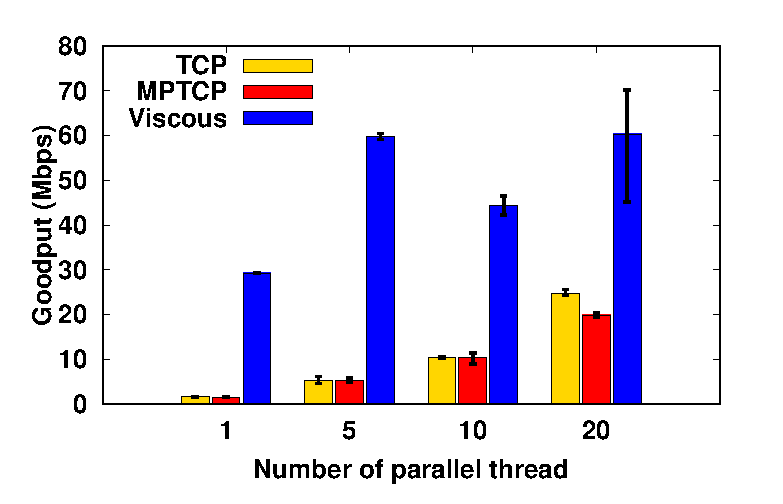
\includegraphics[width=\linewidth]{img/exp7/goodput_20}
			\label{fig:exp7_goodput_320}
			\subcaption{RTT=320ms}
		\end{minipage}
		\caption{\label{fig:exp7_goodput}Experiment 2: Goodput over Topology-1 with Background Traffic}
	\end{center}
\end{figure}



We have performed the similar experiment as given in Experiment 1, however, in this scenario we have considered the performance of the protocols in the presence of  background traffic. To generate background traffic, we have sent continuous HTTP traffic from $H3$ to $H4$ and $H5$ over Topology-1. This traffic is also in the form of the exponential in nature with mean number of packets as $25$ per second. We have plotted the results in Fig.~\ref{fig:exp7_time}, Fig.~\ref{fig:exp7_goodput} and Fig.~\ref{fig:exp7_cwnd}, for average flow completion time, average goodput for the flows and congestion window evolution over time, respectively. Similar to the previous case, we have found that Viscous performs much better than other competing protocols even in the presence of background traffic. Viscous takes less time than other end-to-end protocols, and the drop in performance for Viscous is comparatively less than other protocols when background traffic is present. The effectiveness of Viscous lies in the fact of proper utilization of available capacity over multiple paths, even in the presence of short-lived flows. Fig.~\ref{fig:exp7_cwnd} shows that Viscous can attain a significant boost in congestion window size at both the paths, compared to TCP Cubic. 

%\begin{figure*}[!t]
%    \captionsetup[subfigure]{}
%    \begin{center}
%        \subfloat[\label{fig:exp7_time_16}RTT=16ms]{
%            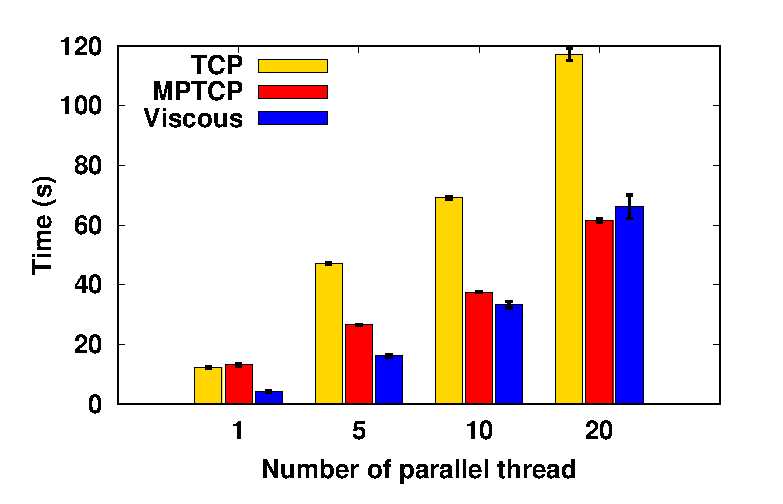
\includegraphics[width=0.24\linewidth]{img/exp7/time_elapsed_1}
%        }
%        \subfloat[\label{fig:exp7_time_80}RTT=80ms]{
%            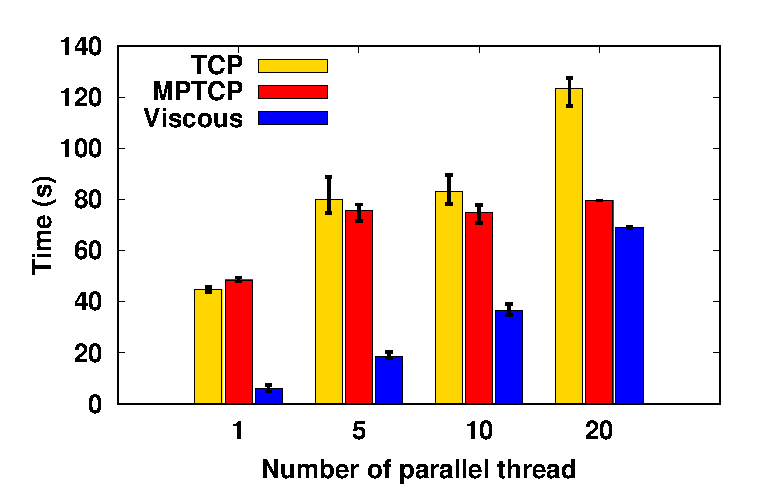
\includegraphics[width=0.24\linewidth]{img/exp7/time_elapsed_5}
%        }
%        \subfloat[\label{fig:exp7_time_160}RTT=160ms]{
%            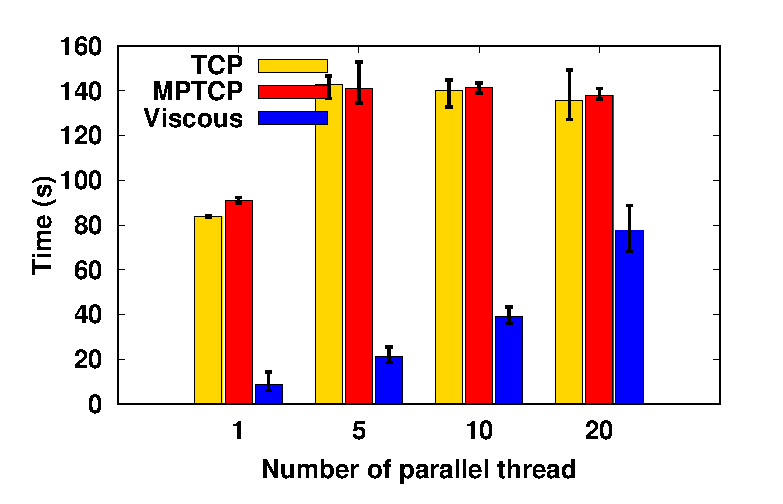
\includegraphics[width=0.24\linewidth]{img/exp7/time_elapsed_10}
%        }
%        \subfloat[\label{fig:exp7_time_320}RTT=320ms]{
%            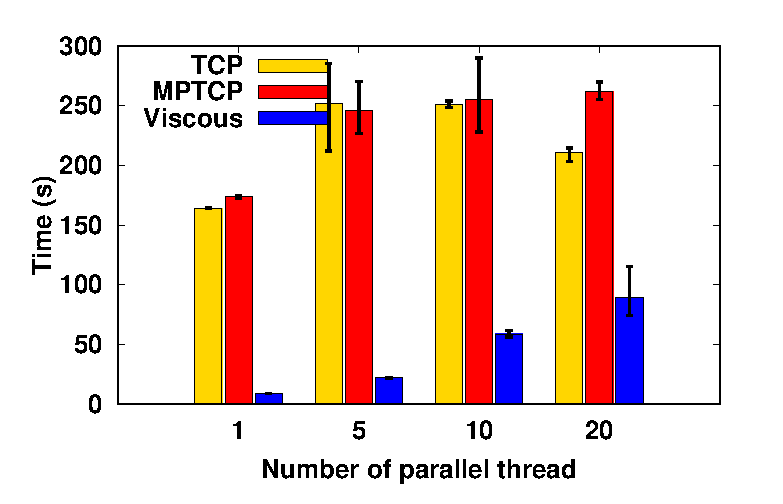
\includegraphics[width=0.24\linewidth]{img/exp7/time_elapsed_20}
%        }
%        \caption{\label{fig:exp7_time}Experiment 2: Flow Completion Time over Topology-1 with Background Traffic}
%    \end{center}
%\end{figure*}
%
%\begin{figure*}[!t]
%    \captionsetup[subfigure]{}
%    \begin{center}
%        \subfloat[\label{fig:exp7_goodput_16}RTT=16ms]{
%            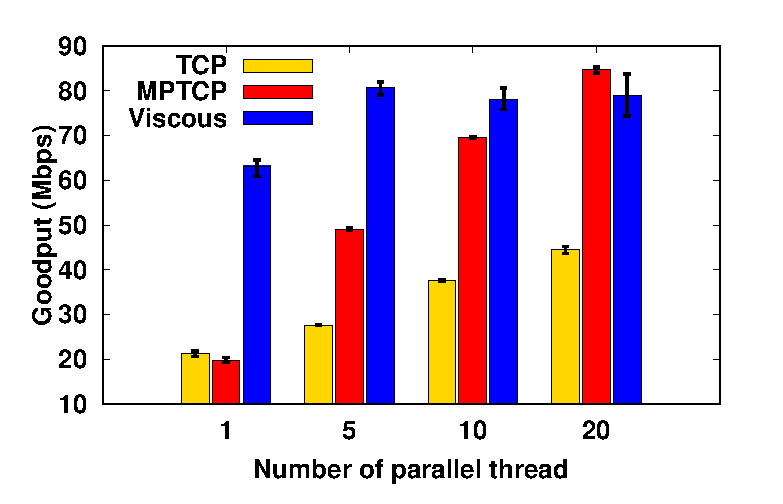
\includegraphics[width=0.24\linewidth]{img/exp7/goodput_1}
%        }
%        \subfloat[\label{fig:exp7_goodput_80}RTT=80ms]{
%            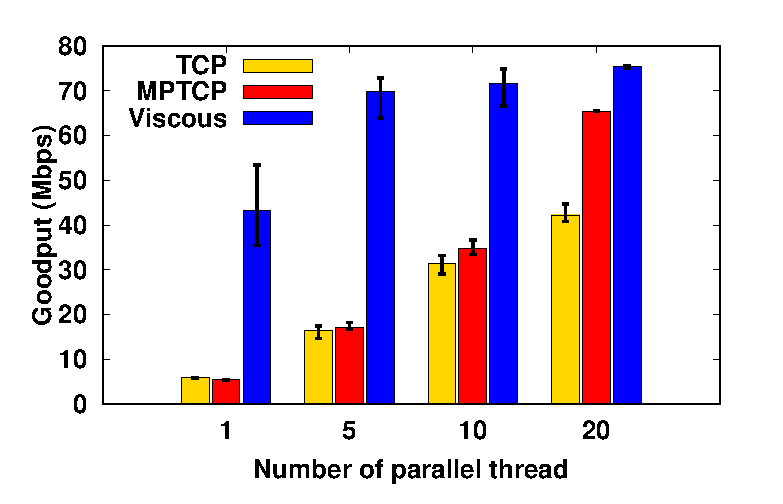
\includegraphics[width=0.24\linewidth]{img/exp7/goodput_5}
%        }
%        \subfloat[\label{fig:exp7_goodput_160}RTT=160ms]{
%            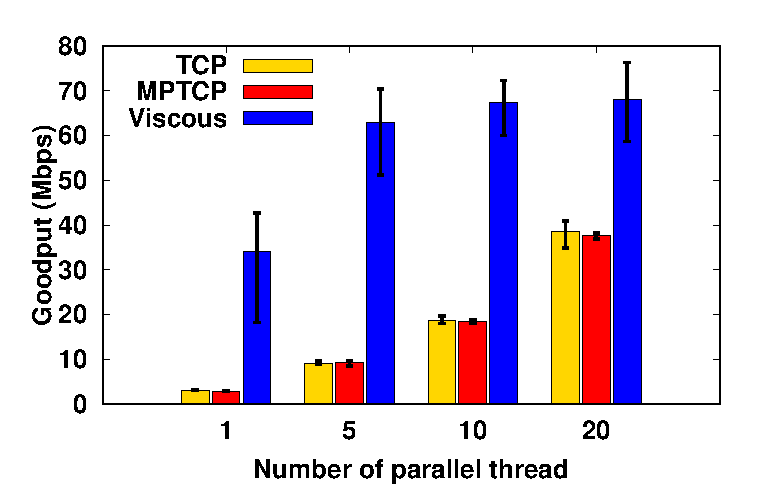
\includegraphics[width=0.24\linewidth]{img/exp7/goodput_10}
%        }
%        \subfloat[\label{fig:exp7_goodput_320}RTT=320ms]{
%            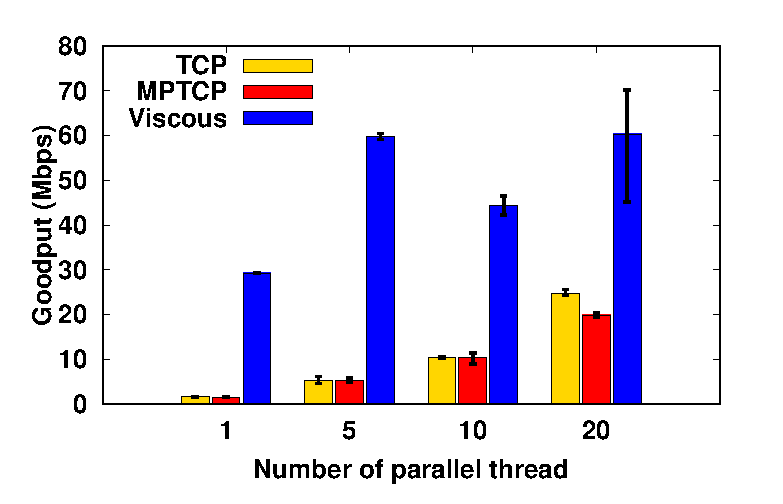
\includegraphics[width=0.24\linewidth]{img/exp7/goodput_20}
%        }
%        \caption{\label{fig:exp7_goodput}Experiment 2: Goodput over Topology-1 with Background Traffic}
%    \end{center}
%\end{figure*}


\subsection{Experiment 3 (Performance over Topology-2 in the Presence of Background Flows)}

%\begin{figure*}[!t]
%	\captionsetup[subfigure]{}
%	\begin{center}
%		\subfloat[\label{fig:exp10_time_16}RTT=16ms]{
%			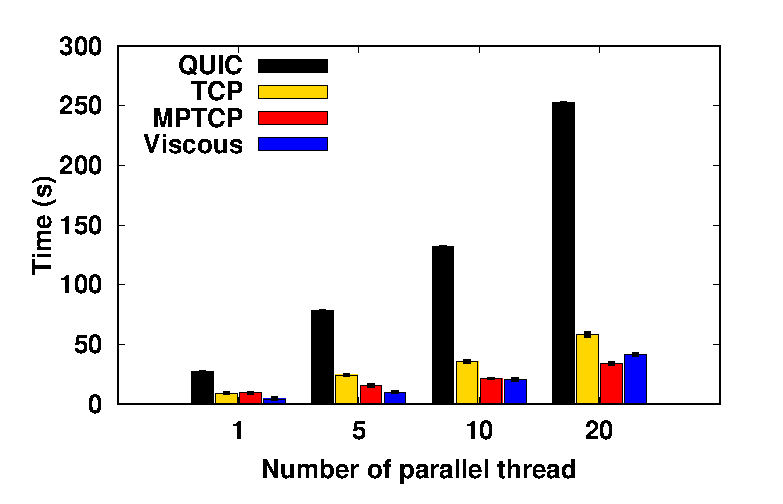
\includegraphics[width=0.24\linewidth]{img/exp10/time_elapsed_1}
%		}
%		\subfloat[\label{fig:exp10_time_80}RTT=80ms]{
%			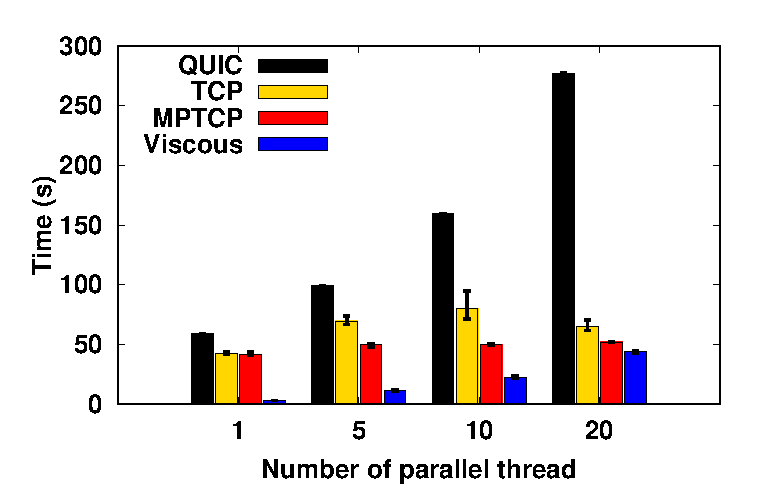
\includegraphics[width=0.24\linewidth]{img/exp10/time_elapsed_5}
%		}
%		\subfloat[\label{fig:exp10_time_160}RTT=160ms]{
%			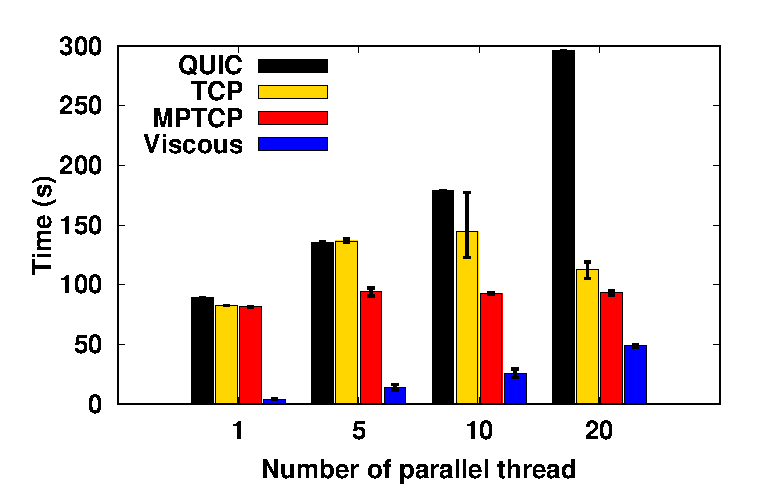
\includegraphics[width=0.24\linewidth]{img/exp10/time_elapsed_10}
%		}
%		\subfloat[\label{fig:exp10_time_320}RTT=320ms]{
%			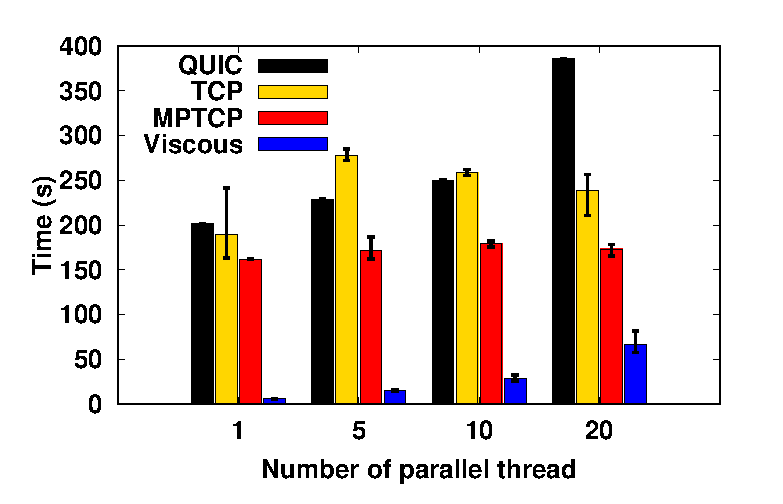
\includegraphics[width=0.24\linewidth]{img/exp10/time_elapsed_20}
%		}
%		\caption{\label{fig:exp10_time}Experiment 3: Flow Completion Time over Topology-2 without Background Traffic}
%	\end{center}
%\end{figure*}
%
%\begin{figure*}[!t]
%	\captionsetup[subfigure]{}
%	\begin{center}
%		\subfloat[\label{fig:exp10_goodput_16}RTT=16ms]{
%			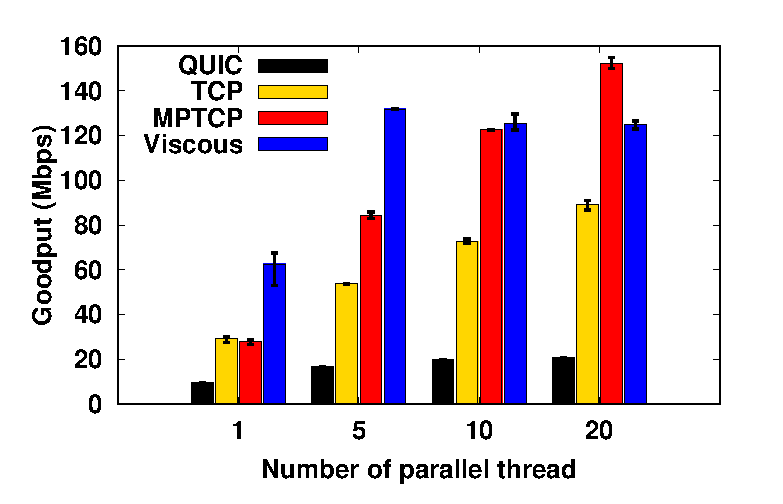
\includegraphics[width=0.24\linewidth]{img/exp10/goodput_1}
%		}
%		\subfloat[\label{fig:exp10_goodput_80}RTT=80ms]{
%			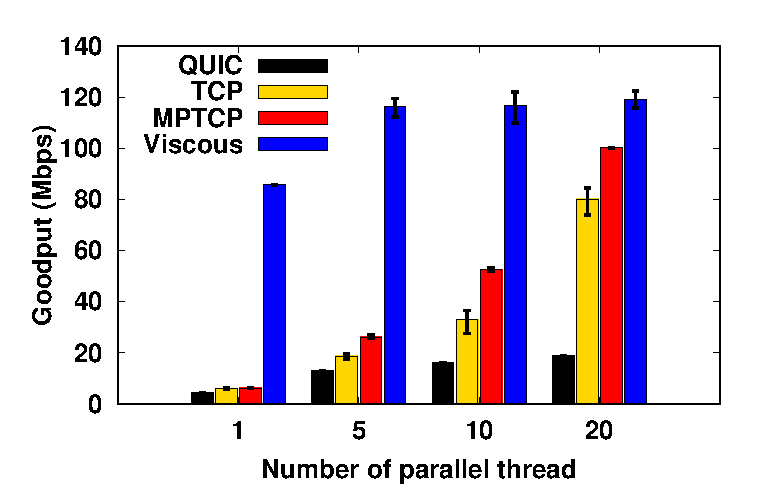
\includegraphics[width=0.24\linewidth]{img/exp10/goodput_5}
%		}
%		\subfloat[\label{fig:exp10_goodput_160}RTT=160ms]{
%			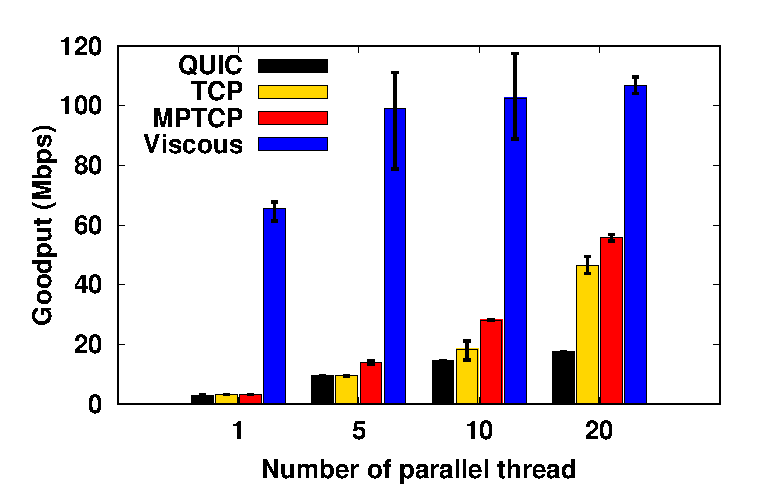
\includegraphics[width=0.24\linewidth]{img/exp10/goodput_10}
%		}
%		\subfloat[\label{fig:exp10_goodput_320}RTT=320ms]{
%			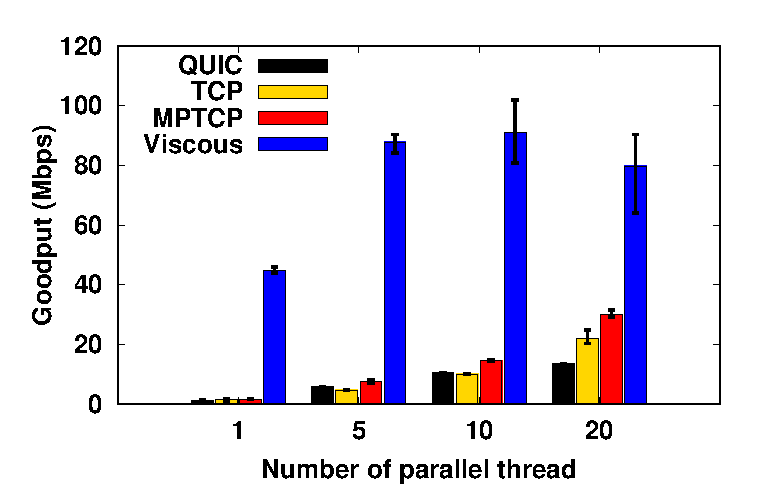
\includegraphics[width=0.24\linewidth]{img/exp10/goodput_20}
%		}
%		\caption{\label{fig:exp10_goodput}Experiment 3: Average Goodput over Topology-2 without Background Traffic}
%	\end{center}
%\end{figure*}

\begin{figure}[!t]
    \begin{center}
        \begin{minipage}{0.45\linewidth}
            \centering
            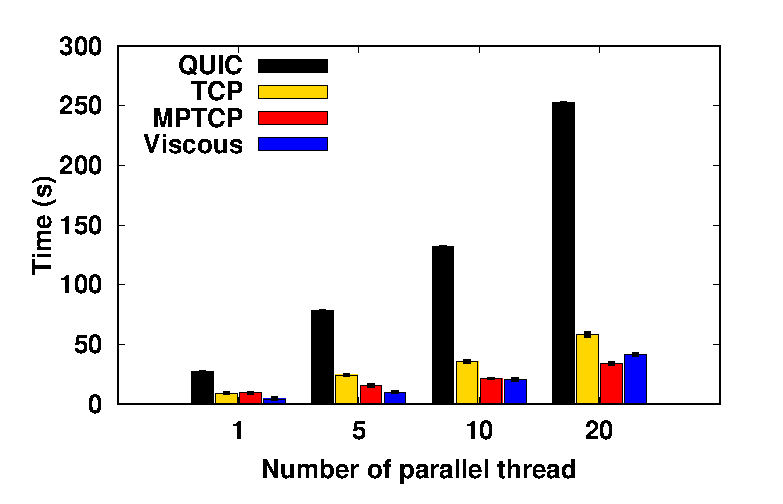
\includegraphics[width=\linewidth]{img/exp10/time_elapsed_1}
            \label{fig:exp10_time_16}
            \subcaption{RTT=16ms}
        \end{minipage}
        \begin{minipage}{0.45\linewidth}
            \centering
            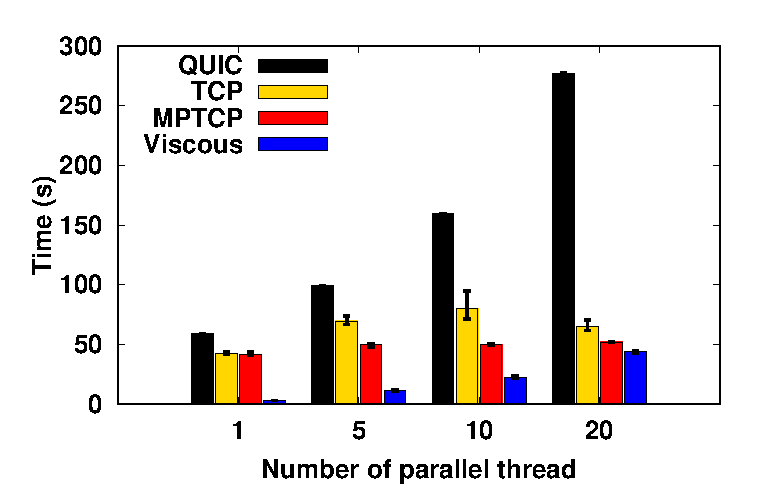
\includegraphics[width=\linewidth]{img/exp10/time_elapsed_5}
            \label{fig:exp10_time_80}
            \subcaption{RTT=80ms}
        \end{minipage}
        \begin{minipage}{0.45\linewidth}
            \centering
            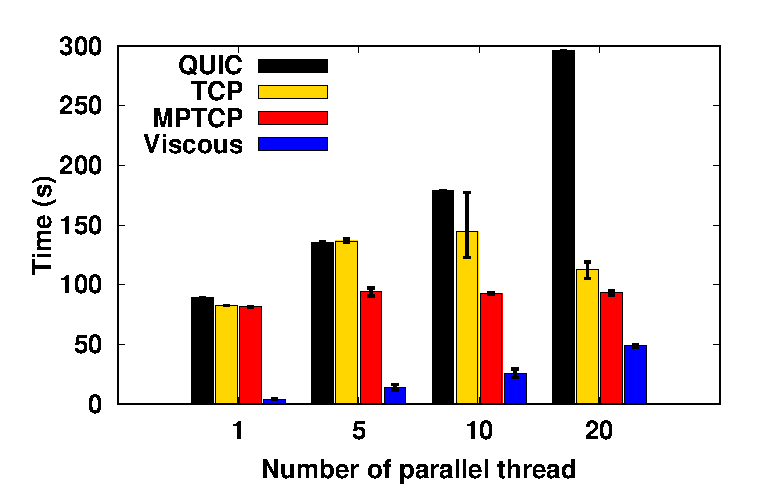
\includegraphics[width=\linewidth]{img/exp10/time_elapsed_10}
            \label{fig:exp10_time_160}
            \subcaption{RTT=160ms}
        \end{minipage}
        \begin{minipage}{0.45\linewidth}
            \centering
            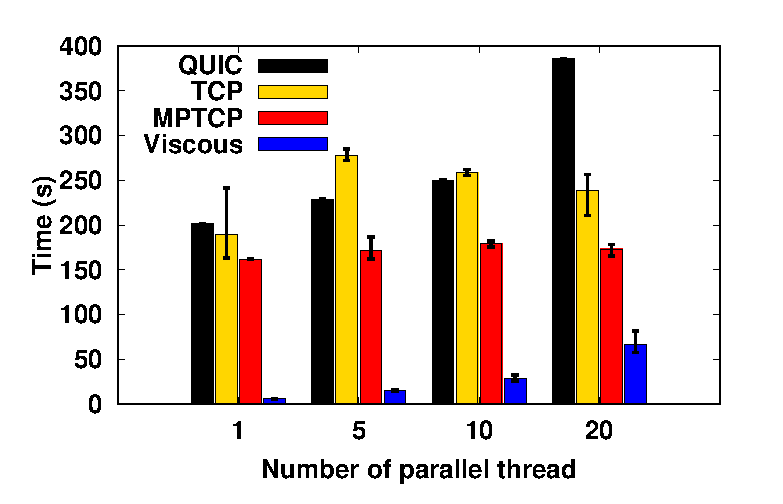
\includegraphics[width=\linewidth]{img/exp10/time_elapsed_20}
            \label{fig:exp10_time_320}
            \subcaption{RTT=320ms}
        \end{minipage}
        \caption{\label{fig:exp10_time}Experiment 3: Flow Completion Time over Topology-2 without Background Traffic}
        \end{center}
    \end{figure}
    
    \begin{figure}[!t]
        \begin{center}
            \begin{minipage}{0.45\linewidth}
                \centering
                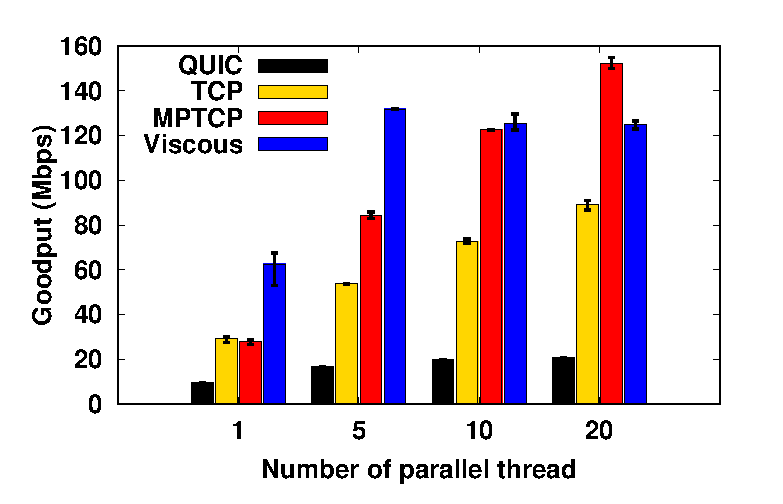
\includegraphics[width=\linewidth]{img/exp10/goodput_1}
                \label{fig:exp10_goodput_16}
                \subcaption{RTT=16ms}
            \end{minipage}
            \begin{minipage}{0.45\linewidth}
                \centering
                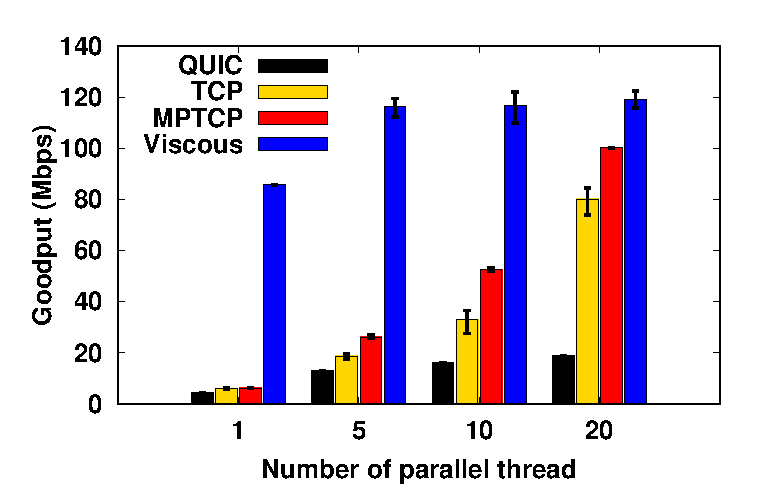
\includegraphics[width=\linewidth]{img/exp10/goodput_5}
                \label{fig:exp10_goodput_80}
                \subcaption{RTT=80ms}
            \end{minipage}
            \begin{minipage}{0.45\linewidth}
                \centering
                \includegraphics[width=\linewidth]{img/exp10/goodput_10}
                \label{fig:exp10_goodput_160}
                \subcaption{RTT=160ms}
            \end{minipage}
            \begin{minipage}{0.45\linewidth}
                \centering
                \includegraphics[width=\linewidth]{img/exp10/goodput_20}
                \label{fig:exp10_goodput_320}
                \subcaption{RTT=320ms}
            \end{minipage}
            \caption{\label{fig:exp10_goodput}Experiment 3: Average Goodput over Topology-2 without Background Traffic}
        \end{center}
    \end{figure}


Next we perform similar experiments over Topology-2, where both the server and the client have multiple interfaces. The results are shown in Fig.~\ref{fig:exp10_time} for average flow completion time, and in Fig.~\ref{fig:exp10_goodput} for average goodput of the flows. Similar to the earlier scenarios, here we observe that Viscous attains better goodput and lower flow completion time compared to QUIC, TCP Cubic and MPTCP. Similar to the previous case, QUIC in this scenario as well, does not perform good for short flows. Although QUIC can multiplex multiple flows coming from the application layer, it maintains flow specific congestion window, resulting in a slow start problem for the flows. Further, QUIC fails to utilize multiple interfaces available in the network which is one of the main reasons behind its poor performance over the test topology. MPTCP suffers from the path imbalance problem as discussed earlier, and TCP Cubic can not utilize multi-homing capacity for the flows. As a consequence, we observe significant performance improvement using Viscous, compared to other protocols. Additionally, we observe that in this scenario, Viscous attains better goodput compared to the goodput over Topology-1, as shown in Fig.~\ref{fig:exp6_goodput}. This indicates that Viscous can properly utilize multihoming of devices, both at the Viscous client as well as at the the Viscous server. 


\subsection{Experiment 4: Performance for Long Flows over a Single Path -- Worst Case Performance of Viscous}


\begin{figure}[!t]
	\centering
	\includegraphics[width=0.5\linewidth]{img/exp1/tcp-mpudp_res}
	\caption{Performance Comparison between Viscous and TCP for Long Flows over a Single Path}
	\label{fig:exp1_singlepath}
\end{figure}


Till now we have tested the performance of Viscous for short-lived flows. To compare its performance for long flows, we have performed this experiment, where we send various size of file from the host $H3$ to the host $H2$ over Topology-1. We plot the time required to transmit a complete file over the network using TCP and Viscous, when both uses only one path in the network. The results are plotted in Fig.~\ref{fig:exp1_singlepath}. From this figure, we observe that the performance of Viscous is almost equal for long flows over a single path, which we consider as the worst case performance for this protocol. This experiment shows that in the worst case, Viscous performs as good as TCP Cubic, however, under the scenarios with multiple short-lived event triggered or user generated flows, Viscous can significantly boost up the end-to-end performance. 


